\begin{figure}[t]
\centering
\resizebox{\columnwidth}{!}{%
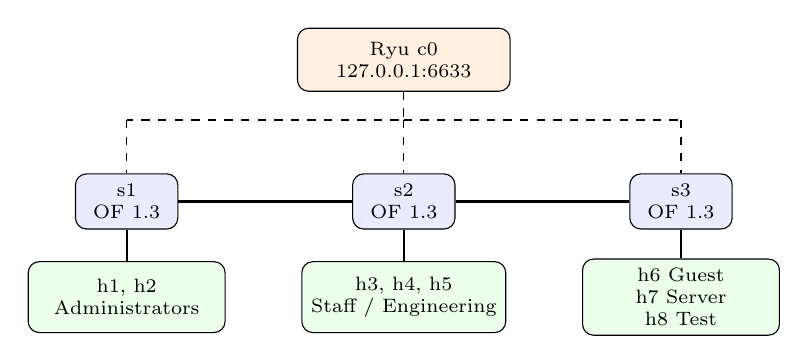
\begin{tikzpicture}[x=11mm,y=9mm,font=\scriptsize,
  sw/.style={draw,rounded corners,minimum width=13mm,minimum height=7mm,fill=blue!8,align=center},
  host/.style={draw,rounded corners,minimum width=25mm,minimum height=9mm,fill=green!8,align=center},
  ctl/.style={draw,rounded corners,minimum width=27mm,minimum height=8mm,fill=orange!12,align=center}]
  \node[ctl] (c) at (3.2,2) {Ryu c0\\127.0.0.1:6633};
  \node[sw] (s1) at (0,0) {s1\\OF 1.3};
  \node[sw] (s2) at (3.2,0) {s2\\OF 1.3};
  \node[sw] (s3) at (6.4,0) {s3\\OF 1.3};
  \coordinate (busl) at (0,1.15); \coordinate (busr) at (6.4,1.15);
  \draw[dashed] (c.south) -- (3.2,1.15) -- (busl);
  \draw[dashed] (3.2,1.15) -- (busr);
  \draw[dashed] (busl) -- (s1.north); \draw[dashed] (3.2,1.15) -- (s2.north);
  \draw[dashed] (busr) -- (s3.north);
  \draw[thick] (s1) -- (s2); \draw[thick] (s2) -- (s3);
  \node[host] (g1) at (0,-1.35) {h1, h2\\Administrators};
  \node[host] (g2) at (3.2,-1.35) {h3, h4, h5\\Staff / Engineering};
  \node[host] (g3) at (6.4,-1.35) {h6 Guest\\h7 Server\\h8 Test};
  \draw[thick] (s1) -- (g1); \draw[thick] (s2) -- (g2); \draw[thick] (s3) -- (g3);
\end{tikzpicture}
}
\caption{NetGuardian topology. Solid lines are data links; dashed lines show controller channels.}
\label{fig:topology}
\end{figure}
